\documentclass[10pt]{article}
\usepackage[top=2cm,bottom=2cm,left=2cm,right=2cm]{geometry}
\usepackage[dvipsnames,svgnames,x11names]{xcolor}
\usepackage{multicol}
\usepackage{graphicx}
\usepackage{amsmath,amssymb,amsfonts}
\usepackage{booktabs}
\usepackage{colortbl}
\usepackage{multirow}
\usepackage{tcolorbox}
\usepackage{enumitem}
\usepackage{titlesec}
\usepackage{float}
\usepackage{hyperref}
\usepackage{tabularx}
\usepackage{subcaption}
\setlength{\parindent}{0pt}
\setlength{\parskip}{6pt}

\graphicspath{{architecture/}}

\begin{document}

%% ============================================================
%% TITLE
%% ============================================================
\begin{center}
{\LARGE\bfseries Structured Knowledge-Enhanced Retrieval for Financial Documents}\\[4pt]
{\large\bfseries Truy xuất tài liệu tài chính tăng cường tri thức cấu trúc}\\[8pt]
{\large Đề xuất nghiên cứu}\\[6pt]
\textit{Benchmark:} $\mathrm{T}^{2}$-RAGBench (EACL 2026) --- FinQA $\cdot$ ConvFinQA $\cdot$ TAT-DQA
\end{center}

\vspace{4pt}
\hrule
\vspace{8pt}

%% ============================================================
%% TÓM TẮT
%% ============================================================
\section*{Tóm tắt}

Truy xuất ngữ cảnh chính xác từ các báo cáo tài chính hỗn hợp văn bản và bảng biểu là bước then chốt trong hệ thống RAG cho lĩnh vực tài chính. Các phương pháp truy xuất hiện tại gặp khó khăn do bỏ qua các đặc trưng ngôn ngữ và ràng buộc toán học vốn có của tài liệu tài chính. Bài báo này phân tích bốn hiện tượng nền tảng gây ra thất bại của các retriever thông thường, từ đó đề xuất GSR (Graph-Structured Retrieval) -- biểu diễn bảng tài chính dưới dạng đồ thị tri thức với các cạnh ràng buộc kế toán, kết hợp cơ chế chấm điểm nhận biết ràng buộc. Ngoài ra, chúng tôi phát triển CACL (Constraint-Aware Contrastive Learning) với kỹ thuật sinh mẫu âm CHAP dựa trên phá vỡ có chủ đích các đẳng thức kế toán. Thực nghiệm trên $\mathrm{T}^{2}$-RAGBench cho thấy GSR vượt trội đáng kể so với các phương pháp dense retrieval tiêu chuẩn.

%% ============================================================
%% 1. GIỚI THIỆU
%% ============================================================
\section{Giới thiệu}

Truy xuất ngữ cảnh phù hợp từ kho tài liệu tài chính là bài toán nền tảng cho các hệ thống RAG trong lĩnh vực này. Đầu vào là câu hỏi tài chính $Q$ và kho gồm $N$ tài liệu $\{D_1, \ldots, D_N\}$, mỗi tài liệu chứa văn bản tự sự, bảng dạng markdown và siêu dữ liệu (tên công ty, năm báo cáo, ngành). Đầu ra là danh sách top-$K$ tài liệu liên quan nhất, đánh giá qua MRR@3, Recall@1/3/5, NDCG@3 theo chuẩn $\mathrm{T}^{2}$-RAGBench~\cite{strich2026t2ragbench}.

Thách thức chính nằm ở tính chất hỗn hợp của thông tin tài chính. Các hệ thống truy xuất tốt nhất hiện nay (Hybrid BM25 với E5-Large Instruct) đạt khoảng 40\% MRR@3 trên FinQA -- khoảng cách đáng kể so với giới hạn trên. Nguyên nhân sâu xa là các phương pháp này chưa khai thác bản chất đặc thù của tài liệu tài chính: bảng số bị làm phẳng thành văn bản, phá hủy quan hệ cha-con và các ràng buộc kế toán.

Phần còn lại của bài báo được tổ chức như sau. Mục 2 trình bày công trình liên quan. Mục 3 phân tích bốn hiện tượng đặc thù của tài liệu tài chính, đồng thời xây dựng khung phân tích lý thuyết nền tảng. Mục 4 trình bày phương pháp GSR. Mục 5 mô tả phương pháp huấn luyện CACL với sinh mẫu âm CHAP. Mục 6 thiết lập thực nghiệm. Mục 7 trình bày kết quả và phân tích.

\subsection{Scope}

Bài báo tập trung vào bài toán \textbf{only retrieval} (truy xuất thuần túy):
\begin{itemize}[leftmargin=*]
    \item \textbf{Đầu vào:} câu hỏi tài chính $Q$ + corpus $N$ documents $\{D_1, \ldots, D_N\}$ (text narrative + markdown table + metadata).
    \item \textbf{Đầu ra:} top-$K$ documents liên quan nhất.
    \item \textbf{Metric:} MRR@3, Recall@1/3/5, NDCG@3.
    \item \textbf{Không bao gồm:} sinh câu trả lời (generation).
\end{itemize}

% \subsection{Khoảng cách hiện tại}

% Hybrid BM25 đạt 35.2\% MRR@3 trên FinQA --- khoảng cách lớn so với Oracle Context. Điều này cho thấy standard retrieval chưa khai thác bản chất đặc thù của tài liệu tài chính.

%% ============================================================
%% 2. CÔNG TRÌNH LIÊN QUAN
%% ============================================================
\section{Công trình liên quan}

\textbf{Truy xuất bảng trong tài liệu tài chính.} HELIOS~\cite{helios2025} sử dụng đồ thị hai phía giữa bảng và văn bản cho câu hỏi đa bước, nhưng không mô hình hóa các ràng buộc kế toán. THYME~\cite{thyme2025} đề xuất ghép nối theo trường (field-aware matching) nhưng chỉ dừng ở mức header. THoRR~\cite{thorr2024} là phương pháp truy xuất hai giai đoạn dựa trên header, thiếu biểu diễn toàn cục các quan hệ số học. ConFIT~\cite{confit2025} sử dụng nhiễu loạn bảo toàn ngữ nghĩa dựa trên từ điển Wikidata, khác với cách tiếp cận dựa trên vi phạm đẳng thức kế toán của chúng tôi.

\textbf{Học đối lập và mẫu âm khó.} DPR~\cite{karpukhin2020dpr} sử dụng mẫu âm ngẫu nhiên và mẫu âm từ BM25. ConFIT chỉ ra lợi ích của mẫu âm được tạo có chủ đích. Tuy nhiên, chưa có phương pháp nào tận dụng các ràng buộc toán học vốn có của bảng tài chính để tạo mẫu âm khó một cách có hệ thống.

\textbf{Lý thuyết ngôn ngữ cho văn bản chuyên ngành.} Halliday~\cite{halliday1994} chỉ ra ngữ nghĩa trong văn bản công thức không nằm ở từ mà ở vị trí cấu trúc. Shannon~\cite{shannon1948} cho thấy entropy trên mỗi token trong văn bản chuyên ngành thấp hơn văn bản thông thường.

%% ============================================================
%% 3. PHÂN TÍCH BẢN CHẤT CỦA TÀI LIỆU TÀI CHÍNH
%% ============================================================
\section{Phân tích bản chất của tài liệu tài chính}

Tài liệu tài chính là hệ thống mã hóa tuân theo các luật ngôn ngữ và ràng buộc toán học bất biến. Bốn hiện tượng sau giải thích tại sao các phương pháp truy xuất thông thường thất bại.

\subsection{Bốn hiện tượng đặc thù}

\textbf{Hiện tượng 1: Tính thể loại đặc thù (Genre-specificity).} Báo cáo tài chính có ba đặc trưng nền tảng:
\begin{itemize}[leftmargin=*]
    \item \textit{Tính lặp lại cao}: cấu trúc câu gần như cố định, làm bão hòa embedding tổng quát.
    \item \textit{Nén từ vựng}: một từ mang nhiều nghĩa kỹ thuật (ví dụ: ``thu nhập'' = thu nhập ròng / thu nhập hoạt động / thu nhập trước thuế).
    \item \textit{Cấu trúc đa phương thức cố định}: $[\text{văn bản}] \to [\text{bảng}] \to [\text{chú thích}] \to [\text{văn bản}]$.
\end{itemize}

\textbf{Hiện tượng 2: Ảo tưởng trùng lặp từ vựng (Lexical Overlap Illusion).} Độ trùng lặp từ vựng cao không đồng nghĩa tương đồng ngữ nghĩa cao. Ngữ nghĩa không nằm trong từ mà nằm trong cấu trúc.

\textbf{Hiện tượng 3: Mất nhất quán toán học (Mathematical Inconsistency).} Báo cáo tài chính bị ràng buộc bởi các phương trình kế toán ẩn:
\begin{equation*}
    \text{Revenue} - \text{COGS} = \text{Gross Profit}, \qquad
    \text{Assets} = \text{Liabilities} + \text{Equity}
\end{equation*}
Khi bảng bị làm phẳng, quan hệ cha-con bị phá hủy.

\textbf{Hiện tượng 4: Nghịch lý mật độ số (Numerical Density Paradox).} Cùng một con số xuất hiện trong nhiều ngữ cảnh. Số liệu vừa là manh mối mạnh vừa là cái bẫy.

\subsection{Bốn định luật ngôn ngữ}

\begin{itemize}[leftmargin=*]
    \item \textbf{Law of Formulaic Encoding} (Halliday 1994): ngữ nghĩa không ở từ mà ở vị trí cấu trúc.
    \item \textbf{Law of Lexical Compression} (Shannon 1948): entropy/token trong văn bản chuyên ngành thấp hơn văn bản thông thường.
    \item \textbf{Law of Numerical Anchoring}: con số là điểm cố định -- thay đổi sẽ hủy ngữ nghĩa.
    \item \textbf{Law of Multi-layered Semantics}: một ngữ cảnh chứa nhiều câu hỏi khác nhau $\Rightarrow$ biểu diễn phải đa diện.
\end{itemize}

\subsection{Ba giả thuyết nghiên cứu}

\begin{itemize}[leftmargin=*]
    \item \textbf{H1 (Tính nhất quán):} Truy xuất vượt trội khi bảo toàn tính tự hợp toán học -- hệ thống kiểm tra được mức thỏa mãn ràng buộc.
    \item \textbf{H2 (Căn chỉnh cấu trúc):} Kết quả tỷ lệ thuận với mức độ căn chỉnh giữa không gian văn bản, cấu trúc và số liệu.
    \item \textbf{H3 (Giá trị mẫu âm khó):} Phân biệt chỉ thực sự khi mô hình đối mặt mẫu nhiễu dựa trên ràng buộc.
\end{itemize}

\subsection{Luận giải từ lý thuyết thông tin}

Thông tin trong bảng tài chính $C$ phân tách thành:
\begin{equation*}
    H(T(C)) = H_T(T) + H_S(T) + H_N(T)
\end{equation*}
với $H_T$: entropy văn bản, $H_S$: entropy cấu trúc (quan hệ cha-con), $H_N$: entropy số liệu. Khi làm phẳng bảng:
\begin{equation*}
    I_{\text{loss}} \geq I_S + I_{\text{discriminative}}(H_N)
\end{equation*}

%% ============================================================
%% 4. PROPOSED METHOD: GSR-CACL
%% ============================================================
\section{GSR: Graph-Structured Retrieval}

Phân tích ở Mục 3 chỉ ra hai thiếu sót cốt lõi của dense retrieval tiêu chuẩn trên tài liệu tài chính. Thứ nhất, phương pháp dựa trên text similarity bỏ qua siêu dữ liệu thực thể, dẫn đến nhầm lẫn Apple 2023 với Apple 2024 hay Microsoft 2023 -- Hiện tượng 4 (Numerical Density Paradox) và Hiện tượng 2 (Lexical Overlap Illusion). Thứ hai, việc làm phẳng bảng phá hủy quan hệ cha-con và các ràng buộc kế toán -- Hiện tượng 3 (Mathematical Inconsistency). Từ nhận định này, bài báo xây dựng một khung nền tảng và phát triển hai đóng góp trên nền tảng đó.

\subsection{Baseline: Text + Entity Retrieval}\label{sec:baseline}

Khung nền tảng bao gồm dense retrieval kết hợp entity signal. Text encoder sử dụng bi-encoder với BAAI/bge-large-en-v1.5~\cite{bge} làm backbone, encode câu hỏi và văn bản thành $\mathbf{q}, \mathbf{d}_{\text{text}} \in \mathbb{R}^d$. Similarity score:
\begin{equation}
    s_{\text{text}}(Q, C) = \cos(\mathbf{q}, \mathbf{d}_{\text{text}})
\end{equation}

Về entity signal, phân tích cho thấy tài liệu tài chính mang siêu dữ liệu thực thể đa chiều (company, year, sector). Khosla et al. ~\cite{khosla2020supcon} đề xuất Supervised Contrastive Learning để học biểu diễn phân biệt đồng tham chiếu. Chúng tôi áp dụng EntitySupConLoss cho company, year, và sector embeddings, được encode qua cùng backbone:
\begin{equation}
    \mathbf{e}_Q = \text{MLP}\big(f_\theta(\text{company}) \oplus f_\theta(\text{year}) \oplus f_\theta(\text{sector})\big)
\end{equation}
với $\oplus$ là concatenation. Entity similarity:
\begin{equation}
    s_{\text{ent}}(Q, C) = \cos(\mathbf{e}_Q, \mathbf{e}_C)
\end{equation}

Khung nền tảng kết hợp hai tín hiệu qua Joint Scorer $\phi_{\text{base}}$:
\begin{equation}
    s_{\text{base}}(Q, C) = \alpha \cdot s_{\text{text}} + \beta \cdot s_{\text{ent}}
\end{equation}
với $\alpha = \text{softplus}(\hat\alpha)$, $\beta = \text{softplus}(\hat\beta)$. Khung này giải quyết vấn đề entity conflation (Hiện tượng 2) nhưng chưa giải quyết được vấn đề bảng phẳng (Hiện tượng 3).

\subsection{Contribution 1: Constraint KG + Edge-aware GAT}\label{sec:gsr}

Phân tích ở Mục 3 chỉ ra rằng bảng tài chính tuân theo các đẳng thức kế toán bất biến: Revenue $-$ COGS $=$ Gross Profit, Assets $=$ Liabilities $+$ Equity. Khi bảng bị làm phẳng thành text, các đẳng thức này bị phá hủy. Contribution 1 biểu diễn bảng dưới dạng Constraint Knowledge Graph và encode bằng edge-aware GAT để đưa tín hiệu cấu trúc vào Joint Scorer.

\subsubsection{Template-Based KG Construction}\label{sec:kg}

\begin{figure}[H]
    \centering
    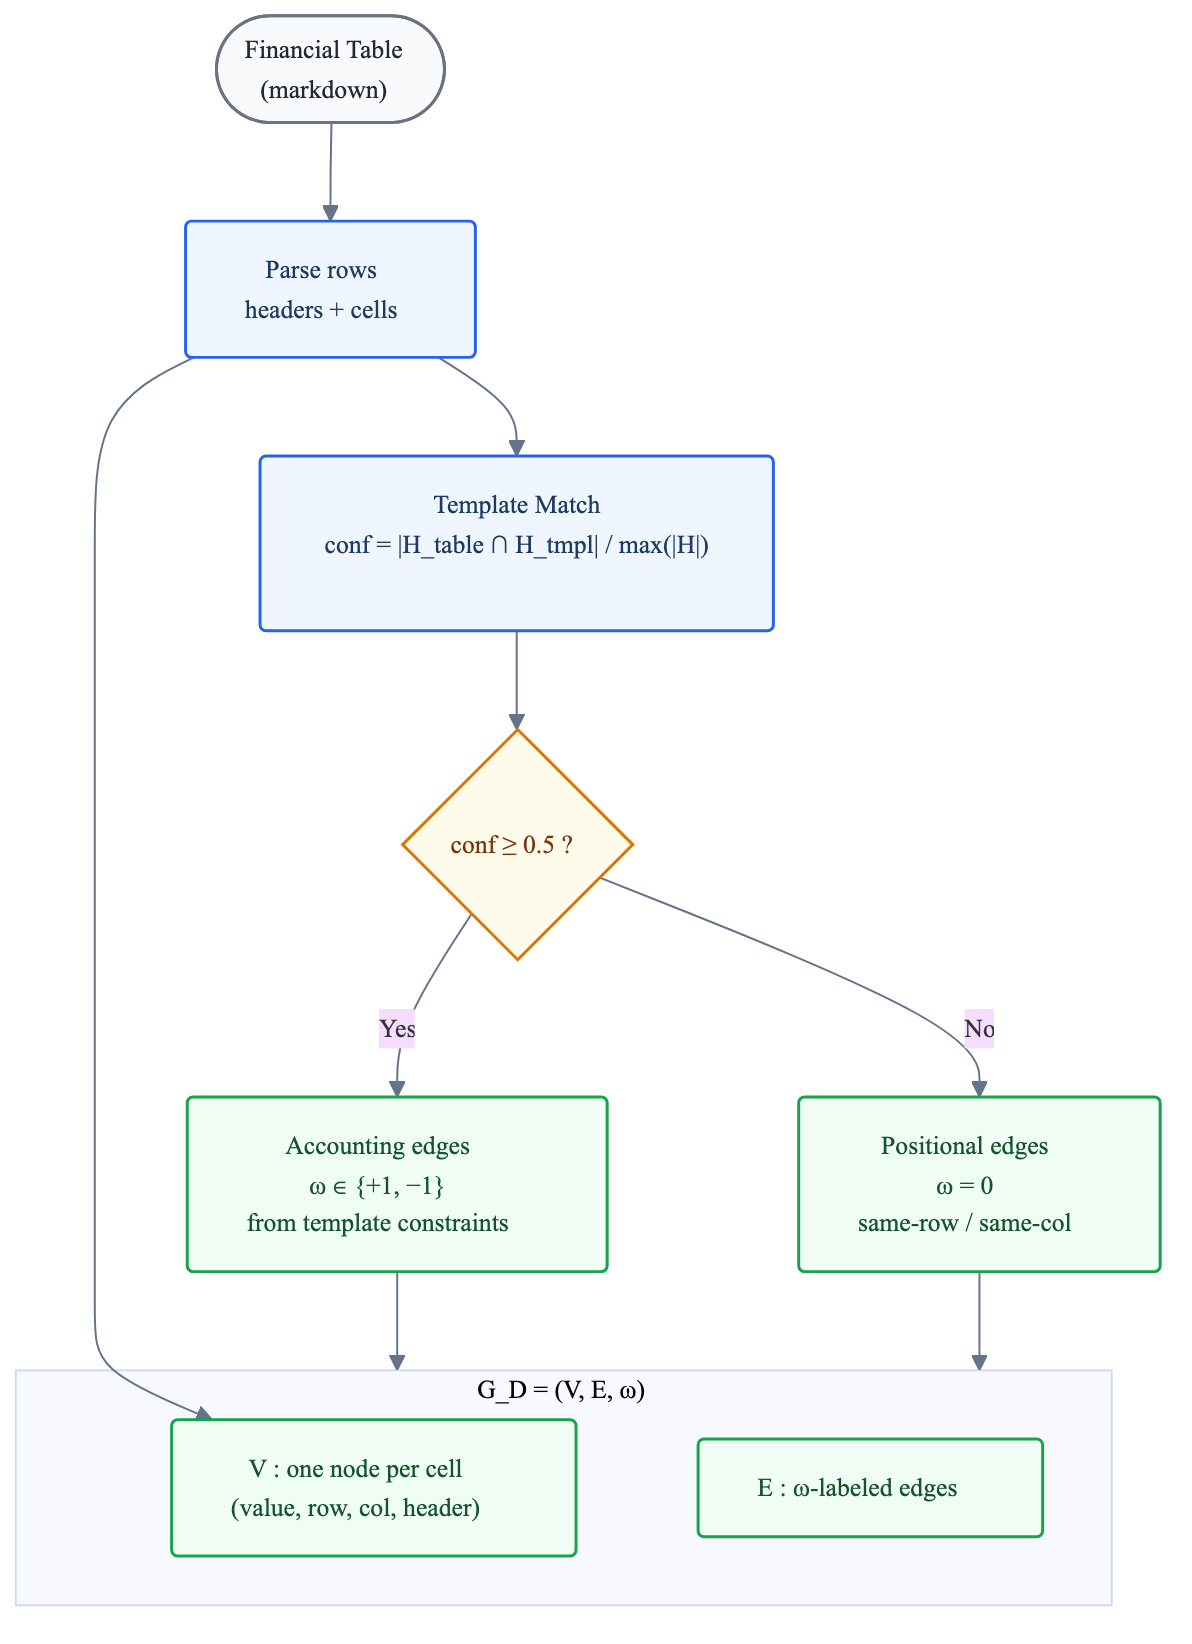
\includegraphics[width=0.7\textwidth]{fig2_kg_construction.png}
    \caption{KG Construction: Bảng markdown $\to$ Parse $\to$ Template Matching $\to$ Constraint Edges $(\omega)$. Fallback: positional edges $(\omega = 0)$.}
    \label{fig:kg}
\end{figure}

Mỗi bảng markdown $T$ chuyển thành $G_D = (\mathcal{V}, \mathcal{E}, \omega)$ qua bốn bước:

\textbf{Bước 1 --- Parse.} Tách header $\mathcal{H}$ và ma trận ô $\{c_{ij}\}$, mỗi ô thành nút $v \in \mathcal{V}$ với $(\text{value}, \text{row}, \text{col}, \text{header})$.

\textbf{Bước 2 --- Template Matching.} So khớp $\mathcal{H}$ với thư viện $\mathcal{T}$ gồm 15 template IFRS/GAAP:
\begin{equation}
    \text{conf}(\mathcal{H}, \tau) = \frac{|\{h \in \mathcal{H} \mid \text{normalize}(h) \in \mathcal{H}_\tau\}|}{\max(|\mathcal{H}|, |\mathcal{H}_\tau|)}
\end{equation}

\begin{table}[H]
\centering\small
\begin{tabular}{ll}
\toprule
Template & Ràng buộc đại diện \\
\midrule
Income Statement & Revenue $-$ COGS $=$ Gross Profit; GP $-$ OpEx $=$ EBIT \\
Balance Sheet (Assets) & Current Assets $+$ Non-Current Assets $=$ Total Assets \\
Balance Sheet (L+E) & Total Liabilities $+$ Equity $=$ Total Assets \\
Cash Flow Statement & OCF $+$ ICF $+$ FCF $=$ Net Cash Flow \\
Revenue by Segment & $\sum_i$ Segment$_i$ $=$ Total Revenue \\
Quarterly Breakdown & Q1 $+$ Q2 $+$ Q3 $+$ Q4 $=$ Annual \\
EBITDA & Revenue $-$ COGS $-$ SG\&A $-$ D\&A $=$ EBITDA \\
EPS & Net Income $/$ Shares Outstanding $=$ EPS \\
\ldots{} (15 templates) & \ldots{} \\
\bottomrule
\end{tabular}
\end{table}

\textbf{Bước 3 --- Edge Construction.} Nếu $\text{conf} \geq 0.5$, tạo cạnh accounting:
\begin{equation}
    \omega_{uv} = \begin{cases} +1 & \text{additive (cha = tổng các con)} \\ -1 & \text{subtractive (cha = một con trừ đi)} \end{cases}
\end{equation}

\textbf{Bước 4 --- Fallback.} Nếu $\text{conf} < 0.5$, cạnh positional $\omega = 0$.

\textbf{Coverage:} $\sim$80--90\% FinQA/ConvFinQA; $\sim$70\% TAT-DQA.

\subsubsection{Edge-Aware GAT Encoder}\label{sec:gat}

\begin{figure}[H]
    \centering
    \begin{minipage}[b]{0.55\textwidth}
        \centering
        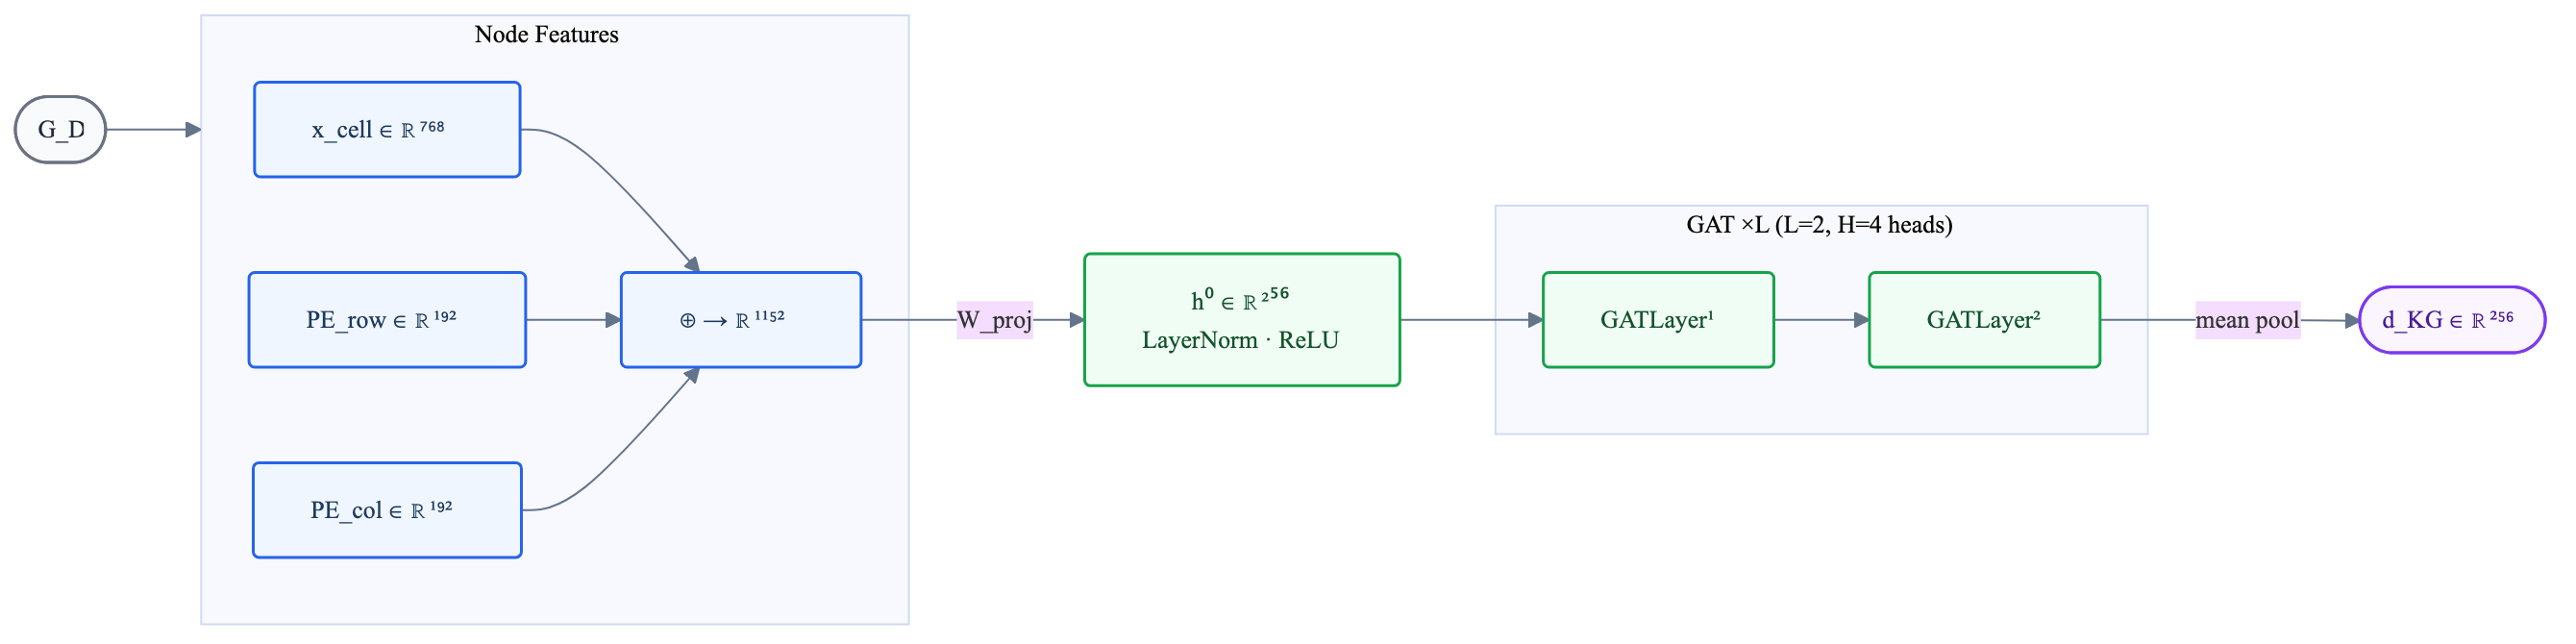
\includegraphics[width=\textwidth]{fig3_gat_encoder.png}
        \captionof{figure}{GAT Encoder overview.}
    \end{minipage}
    \hfill
    \begin{minipage}[b]{0.42\textwidth}
        \centering
        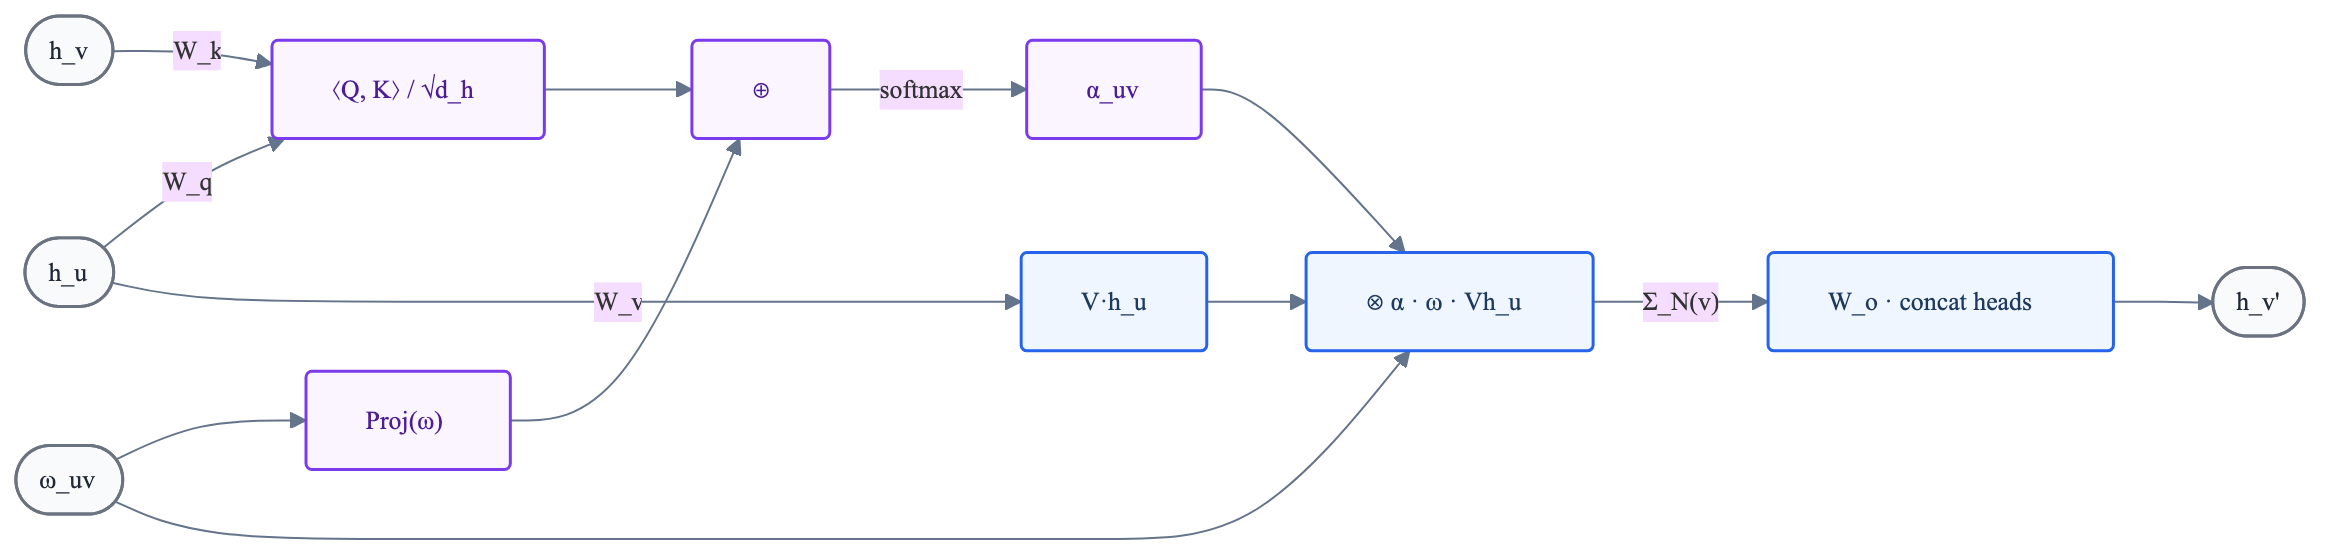
\includegraphics[width=\textwidth]{fig3b_edge_attention.png}
        \captionof{figure}{Edge-aware attention.}
    \end{minipage}
    \caption{GAT Encoder. (a)~Node features $\to$ $L=2$ edge-aware GAT layers $\to$ mean-pooled $\mathbf{d}_{\text{KG}}$. (b)~Attention bias bởi $\omega_{uv}$.}
    \label{fig:gat}
\end{figure}

\textbf{Node Features:}
\begin{equation}
    \mathbf{x}_v = f_\theta(\text{cell\_text}_v) \oplus \text{PE}_{\text{row}}(r) \oplus \text{PE}_{\text{col}}(c) \in \mathbb{R}^{d + 2p}
\end{equation}
\begin{equation}
    \mathbf{h}_v^{(0)} = \text{ReLU}\big(\text{LayerNorm}(W_{\text{proj}}\, \mathbf{x}_v)\big)
\end{equation}

\textbf{Edge-Aware Attention (layer $l$, head $k$):}
\begin{equation}
    e_{uv}^{(k)} = \frac{\langle W_q^{(k)} \mathbf{h}_u^{(l)},\; W_k^{(k)} \mathbf{h}_v^{(l)} \rangle}{\sqrt{d_k}} + \text{Proj}(\omega_{uv})
\end{equation}
\begin{equation}
    \alpha_{uv}^{(k)} = \frac{\exp(e_{uv}^{(k)})}{\sum_{w \in \mathcal{N}(v)} \exp(e_{wv}^{(k)})}
\end{equation}

\textbf{Message Passing:}
\begin{equation}
    \mathbf{h}_v^{(l+1)} = W_o \bigg[\Big\|_{k=1}^{H} \sum_{u \in \mathcal{N}(v)} \alpha_{uv}^{(k)} \cdot \omega_{uv} \cdot W_v^{(k)} \mathbf{h}_u^{(l)} \bigg] + \mathbf{h}_v^{(l)}
\end{equation}

\textbf{Graph-Level Representation:}
\begin{equation}
    \mathbf{d}_{\text{KG}} = \frac{1}{|\mathcal{V}|} \sum_{v \in \mathcal{V}} \mathbf{h}_v^{(L)} \in \mathbb{R}^{h_{\text{dim}}}
\end{equation}
với $L = 2$ layers, $H = 4$ heads, $h_{\text{dim}} = 256$.

\subsubsection{Constraint Scoring}

Từ Constraint KG $G_D$, đo mức tuân thủ các đẳng thức kế toán:
\begin{equation}
    \text{CS}(G_D) = \frac{1}{|\mathcal{E}_c|} \sum_{(u,v,\omega) \in \mathcal{E}_c} \exp\!\Big(-\frac{|\omega \cdot v_u - v_v|}{\max(|v_v|, \varepsilon)}\Big) \in (0, 1]
\end{equation}

Điểm này khác zero chỉ khi tài liệu thực sự tuân theo ràng buộc -- phân biệt được tài liệu có cấu trúc hợp lệ với tài liệu ngẫu nhiên.

\subsection{Joint Scorer $\phi_\theta$: Kết hợp ba tín hiệu}\label{sec:scorer}

\begin{figure}[H]
    \centering
    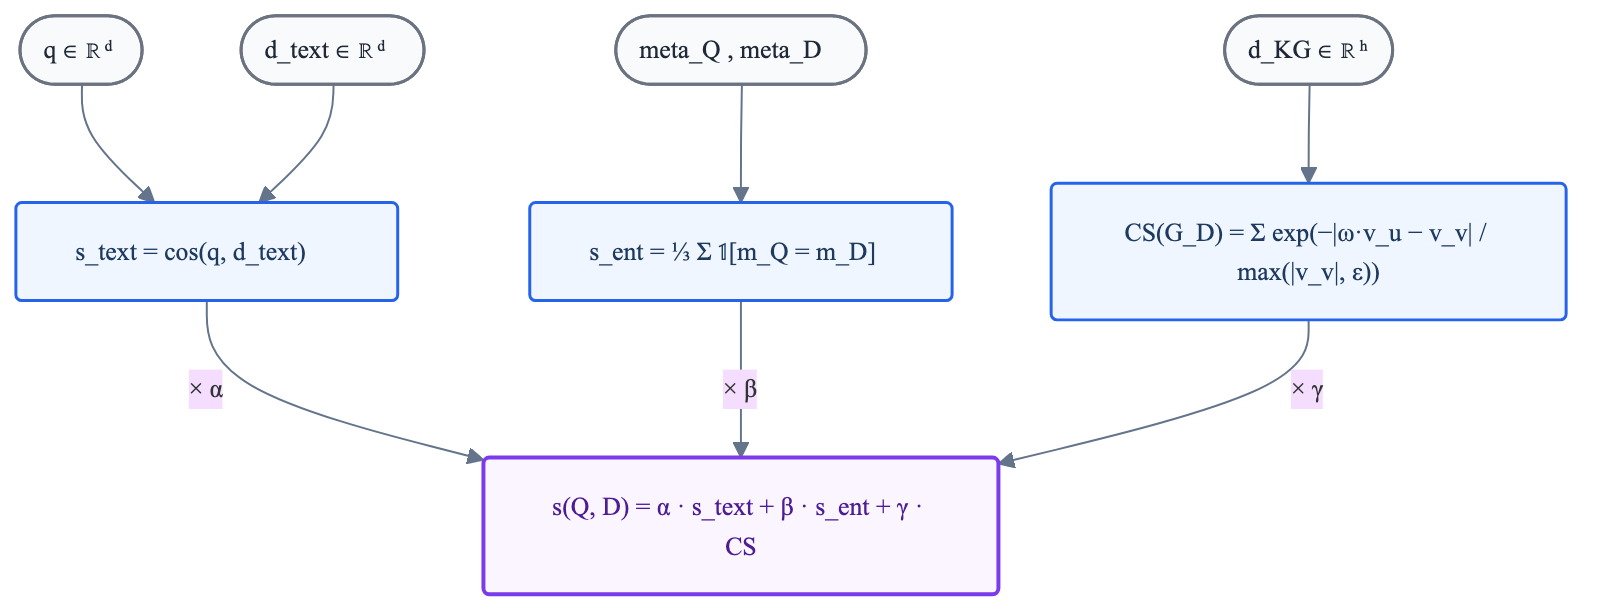
\includegraphics[width=0.6\textwidth]{fig4_joint_scorer.png}
    \caption{Joint Scorer $\phi_\theta$: ba tín hiệu bổ trợ $\to$ trọng số học được $(\alpha, \beta, \gamma)$.}
    \label{fig:scorer}
\end{figure}

GSR nâng cấp Joint Scorer từ $\phi_{\text{base}}$ lên $\phi_\theta$ bằng cách thêm constraint signal:
\begin{equation}\label{eq:joint}
    s(Q, C) = \alpha \cdot s_{\text{text}}(Q, C) + \beta \cdot s_{\text{ent}}(Q, C) + \gamma \cdot \text{CS}(G_D)
\end{equation}
với $\alpha, \beta, \gamma = \text{softplus}(\hat\cdot)$, khởi tạo $\alpha_0 = 0.5$, $\beta_0 = 0.3$, $\gamma_0 = 0.2$.

\textbf{Ký hiệu:}

\begin{table}[H]
\centering\small
\begin{tabular}{cl}
\toprule
Ký hiệu & Ý nghĩa \\
\midrule
$\mathbf{q} \in \mathbb{R}^d$ & Embedding câu hỏi \\
$\mathbf{d}_{\text{text}} \in \mathbb{R}^d$ & Embedding văn bản \\
$G_D = (\mathcal{V}, \mathcal{E}, \omega)$ & Constraint KG của bảng $T$ \\
$\mathbf{d}_{\text{KG}} \in \mathbb{R}^h$ & Graph embedding sau GAT \\
$\phi_\theta$ & Joint Scorer \\
$s(Q, C)$ & Điểm liên quan tổng hợp \\
$\alpha, \beta, \gamma$ & Trọng số học được (softplus-constrained) \\
$\omega_{uv} \in \{+1, -1, 0\}$ & Trọng số cạnh kế toán \\
\bottomrule
\end{tabular}
\end{table}

\subsection{Contribution 2: CHAP Negatives (Đang hoàn thiện)}\label{sec:chap-overview}

Khung nền tảng và Contribution 1 giải quyết vấn đề inference. Contribution 2 bổ trợ cho giai đoạn huấn luyện bằng cách tạo hard negatives dựa trên vi phạm ràng buộc kế toán. Chi tiết về CHAP, hàm mất mát ConstraintViolation, và curriculum training được trình bày ở Mục 5.

\section{CACL: Constraint-Aware Contrastive Learning (Đang hoàn thiện)}

CACL bổ trợ cho GSR trong giai đoạn huấn luyện. Phương pháp huấn luyện bao gồm sinh mẫu âm CHAP, hàm mất mát ConstraintViolation, và three-stage curriculum.

\subsection{CHAP: Constraint-Aware Hard Negative Generation}\label{sec:chap}

\begin{figure}[H]
    \centering
    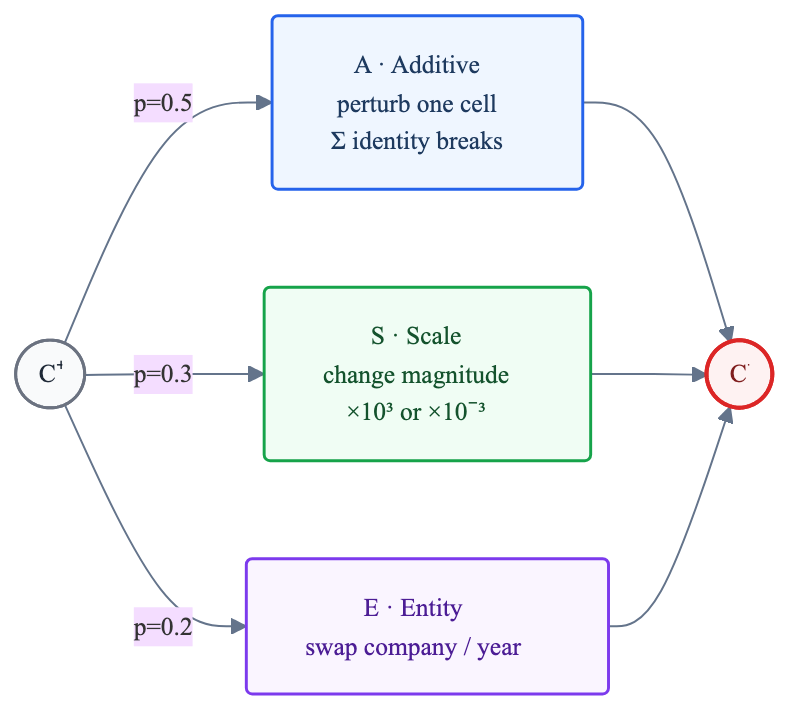
\includegraphics[width=0.7\textwidth]{fig5_chap.png}
    \caption{CHAP Negative Sampler: ba kiểu nhiễu loạn, mỗi kiểu phá vỡ đúng một đẳng thức kế toán.}
    \label{fig:chap}
\end{figure}

CHAP tạo mẫu âm $C^-$ từ tài liệu dương $C^+$ bằng phá vỡ đúng một đẳng thức kế toán:

\begin{table}[H]
\centering\small
\begin{tabular}{llll}
\toprule
Kiểu & Phép biến đổi & Ràng buộc bị vi phạm & Xác suất \\
\midrule
\textbf{A} (Additive) & Thay đổi 1 ô con, giữ nguyên ô tổng & $\sum_i v_{\text{child}_i} \neq v_{\text{parent}}$ & $p = 0.5$ \\
\textbf{S} (Scale) & Biến đổi bậc đại lượng ($\times 10^3$) & Tỷ lệ giữa các ô bị phá vỡ & $p = 0.3$ \\
\textbf{E} (Entity) & Hoán đổi company/year trong metadata & Sai khớp thực thể/thời gian & $p = 0.2$ \\
\bottomrule
\end{tabular}
\end{table}

\textbf{Tính chất Zero-Sum:} Mỗi $C^-$ chỉ khác $C^+$ đúng một thành phần $\Rightarrow$ ``rất giống nhưng chắc chắn sai''.

\subsection{Training Objective: $\mathcal{L}_{\text{CACL}}$}\label{sec:loss}

\begin{figure}[H]
    \centering
    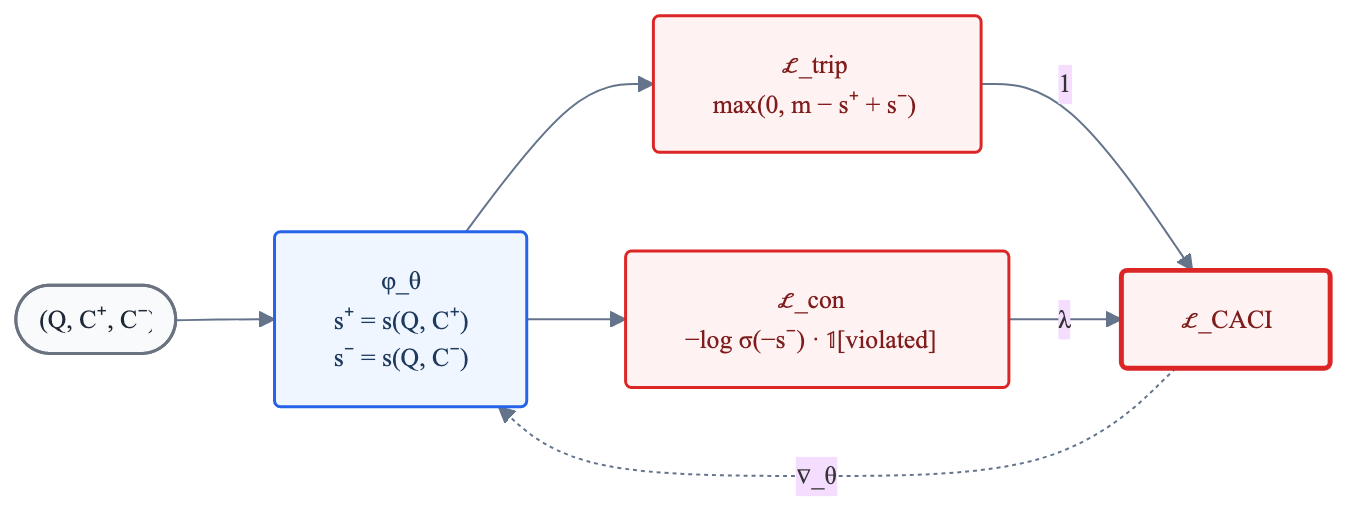
\includegraphics[width=0.7\textwidth]{fig6_cacl_loss.png}
    \caption{CACL Training Objective: margin-based triplet loss + constraint violation penalty.}
    \label{fig:loss}
\end{figure}

\textbf{Triplet Loss:}
\begin{equation}
    \mathcal{L}_{\text{triplet}} = \\frac{1}{N} \sum_{i=1}^{N} \max\!\big(0,\; m - s(Q_i, C_i^+) + s(Q_i, C_i^-)\big)
\end{equation}

\textbf{Constraint Violation Loss:}
\begin{equation}
    \mathcal{L}_{\text{constraint}} = -\\frac{1}{N} \sum_{i=1}^{N} \mathbb{1}[\text{violated}(C_i^-, G_{C_i^-})] \cdot \log\sigma(-s(Q_i, C_i^-))
\end{equation}

\textbf{Trực giác:} $\mathcal{L}_{\text{triplet}}$ dạy phân biệt đúng/sai; $\mathcal{L}_{\text{constraint}}$ dạy \textit{tại sao} sai.

\subsection{Three-Stage Curriculum Training}\label{sec:curriculum}

\begin{figure}[H]
    \centering
    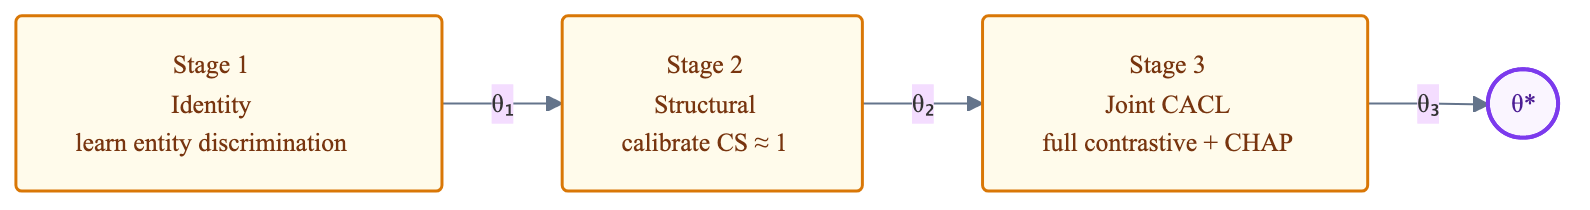
\includegraphics[width=0.7\textwidth]{fig7_curriculum.png}
    \caption{Three-Stage Curriculum: $\theta_1 \to \theta_2 \to \theta_3 = \theta^*$.}
    \label{fig:curriculum}
\end{figure}

\begin{table}[H]
\centering\small
\begin{tabular}{llll}
\toprule
Giai đoạn & Module huấn luyện & Mục tiêu & Loss \\
\midrule
Stage 1: Identity & $f_\theta$ + $\phi_\theta$ & Phân biệt $(company, year)$ & $\mathcal{L}_{\text{triplet}}$ (chỉ $s_{\text{text}} + s_{\text{ent}}$) \\
Stage 2: Structural & $f_\theta$ + GAT + $\phi_\theta$ & Hiệu chuẩn $\text{CS} \approx 1$ cho tài liệu hợp lệ & $\mathcal{L}_{\text{triplet}}$ (full $s$) \\
Stage 3: Joint CACL & $f_\theta$ + GAT + $\phi_\theta$ + CHAP & Tối ưu với mẫu âm khó & $\mathcal{L}_{\text{CACL}}$ \\
\bottomrule
\end{tabular}
\end{table}

%% ============================================================
%% 5. EXPERIMENTAL SETUP
%% ============================================================
\section{Experimental Setup}

\subsection{Datasets}

\begin{table}[H]
\centering\small
\begin{tabular}{lrrrr}
\toprule
Subset & Documents & QA Pairs & Avg. Token/Doc & Domain \\
\midrule
FinQA~\cite{chen2021finqa} & 2,789 & 8,281 & 950.4 & S\&P 500 reports \\
ConvFinQA~\cite{chen2022convfinqa} & 1,806 & 3,458 & 890.9 & S\&P 500 (conversational) \\
TAT-DQA~\cite{zhu2022tatdqa} & 2,723 & 11,349 & 915.3 & Diverse reports \\
\midrule
\textbf{Tổng} & \textbf{7,318} & \textbf{23,088} & \textbf{924.2} & \\
\bottomrule
\end{tabular}
\end{table}

\subsection{Baselines}

\begin{table}[H]
\centering\small
\begin{tabular}{ll}
\toprule
Nhóm & Phương pháp \\
\midrule
Giới hạn & Oracle Context (giới hạn trên), Pretrained-Only \\
Basic RAG & Base-RAG~\cite{karpukhin2020dpr}, Hybrid BM25 \\
LLM-Enhanced & HyDE, Summarization, SumContext (yêu cầu QwQ-32B) \\
Table-Aware & THoRR~\cite{thorr2024}, ConFIT~\cite{confit2025} \\
\midrule
\textbf{GSR (bài báo này)} & Inference-only: Constraint KG + GAT + Joint Scorer \\
GSR + CACL & Huấn luyện với CHAP negatives (đang hoàn thiện) \\
\bottomrule
\end{tabular}
\end{table}

\subsection{Evaluation Metrics}

\begin{table}[H]
\centering\small
\begin{tabular}{lll}
\toprule
Metric & Ý nghĩa & Lý do lựa chọn \\
\midrule
\textbf{MRR@3} & Mean Reciprocal Rank at $k=3$ & Metric chính của $\mathrm{T}^{2}$-RAGBench \\
\textbf{Recall@3} & Tỷ lệ có GT trong top-3 & Đánh giá coverage \\
\textbf{NDCG@3} & Normalized DCG at $k=3$ & Đánh giá thứ hạng có trọng số \\
Recall@1, Recall@5 & Supplementary recall & Phân tích chi tiết chất lượng \\
\bottomrule
\end{tabular}
\end{table}

\subsection{Implementation Details}

\begin{table}[H]
\centering\small
\begin{tabular}{ll}
\toprule
Tham số & Giá trị \\
\midrule
Text encoder & BAAI/bge-large-en-v1.5 ($d = 1024$) \\
Fine-tuning strategy & LoRA ($r = 16$, $\alpha = 32$) \\
GAT layers / heads / hidden & $L = 2$ / $H = 4$ / $h_{\text{dim}} = 256$ \\
Template library size & $|\mathcal{T}| = 15$ IFRS/GAAP templates \\
Template matching threshold & $\tau_{\min} = 0.5$ \\
Training stages & Stage 1: 3 epochs / Stage 2: 3 / Stage 3: 5 \\
Batch size & 8 (T4 16GB) hoặc 16 (A100) \\
Learning rate & $2 \times 10^{-5}$ (AdamW, cosine schedule) \\
Margin $m$ & 0.3; $\lambda$ & 0.5 \\
CHAP ratios (A/S/E) & 0.5 / 0.3 / 0.2 \\
Hardware & NVIDIA T4 16GB (Kaggle) hoặc A100 40GB \\
\bottomrule
\end{tabular}
\end{table}

\begin{table}[H]
\centering\small
\begin{tabular}{llr}
\toprule
Component & Complexity & Per-document \\
\midrule
KG Construction & $O(|\mathcal{V}|)$ & $\sim$57 cells avg \\
GAT Encoding & $O(|\mathcal{V}| \cdot |\mathcal{E}|)$ & $|\mathcal{V}| \approx 57$, $|\mathcal{E}| \approx 10$ \\
Constraint Scoring & $O(|\mathcal{E}_c|)$ & $\sim$5--10 edges \\
CHAP Generation & $O(|\mathcal{V}|)$ & Pre-generated offline \\
\midrule
\textbf{Inference overhead} & & $\sim$1.2--1.4$\times$ vs Base-RAG \\
\bottomrule
\end{tabular}
\end{table}

%% ============================================================
%% 6. RESULTS & ANALYSIS
%% ============================================================
\section{Results \& Analysis}

\subsection{Main Results}

\textbf{Exp 1 --- So sánh toàn diện với baselines.}


\begin{table*}[h]
\centering
\small\setlength{\tabcolsep}{4pt}
\begin{tabular}{ll|c|cc|cc|cc}
\toprule
\multirow{2}{*}{\textbf{Phương pháp}} & \multirow{2}{*}{\textbf{Mô hình nhúng (Retriever)}} & \textbf{Support} & \multicolumn{2}{c|}{\textbf{FinQA}} & \multicolumn{2}{c|}{\textbf{ConvFinQA}} & \multicolumn{2}{c}{\textbf{TAT-DQA}} \\
 & & \textbf{} & MRR@3 & R@3 & MRR@3 & R@3 & MRR@3 & R@3 \\
\midrule
\multicolumn{9}{c}{\textbf{Truy xuất trực tiếp}} \\
\midrule
Base-RAG & E5-Large Instruct & --- & 38.7 & 49.7 & 42.4 & 53.8 & 25.2 & 28.4 \\
Hybrid BM25 & E5-Large Instruct + BM25 & --- & 40.0 & 53.0 & 43.6 & 57.2 & \textbf{29.3} & \textbf{44.4} \\
Reranker & E5-Large Instruct + Reranker & --- & 29.0 & 36.2 & 32.7 & 40.5 & 22.9 & 28.4 \\
\midrule
\multicolumn{9}{c}{\textbf{Sử dụng LLM tiền xử lý ngữ cảnh}} \\
\midrule
HyDE & E5-Large Instruct & QwQ-32B & 35.4 & 45.7 & 39.9 & 50.9 & 20.8 & 26.7 \\
Summarization & E5-Large Instruct & QwQ-32B & \textbf{47.3} & \textbf{59.5} & \textbf{52.2} & \textbf{63.8} & 24.7 & 31.5 \\
SumContext & E5-Large Instruct & QwQ-32B & \textbf{47.3} & 59.4 & \textbf{52.2} & \textbf{63.8} & 24.8 & 31.4 \\
\midrule
Ours &  &  & \textbf{60.4} & \textbf{65.0} & \textbf{65.94} & \textbf{70.99} & \textbf{31.1}  & \textbf{39.42} \\
\midrule
\bottomrule
\end{tabular}
\caption{Đánh giá năng lực của Pha Truy xuất. Các chỉ số được hợp nhất từ kết quả thực nghiệm chung. Cột "Support" chỉ ra phương pháp có yêu cầu một mô hình ngôn ngữ tái cấu trúc dữ liệu trước khi thực hiện nhúng vector hay không.}
\label{tab:retrieval_architecture}
\end{table*}
% \begin{table*}[h!]
% \centering
% \tiny\setlength{\tabcolsep}{3pt}
% \begin{tabular}{ll|ccc|ccc|ccc|ccc}
% \toprule
%  & \multirow{2}{*}{Phương pháp} & \multicolumn{3}{c|}{FinQA} & \multicolumn{3}{c|}{ConvFinQA} & \multicolumn{3}{c|}{TAT-DQA} & \multicolumn{3}{c}{W. Avg} \\
%  & & MRR@3 & R@3 & NDCG@3 & MRR@3 & R@3 & NDCG@3 & MRR@3 & R@3 & NDCG@3 \\
% \midrule
% % \multicolumn{14}{l}{\textit{Giới hạn}} \\
% %  & Oracle Context & 100 & 100 & 100 & 100 & 100 & 100 & 100 & 100 & 100 \\
% % \multicolumn{14}{l}{\textit{Baselines}} \\
% %  & BM25 & 28.0 & 36.0 & --- & 24.0 & 33.0 & --- & 26.0 & 34.5 & --- \\
% %  & Hybrid BM25 & 35.2 & 45.0 & --- & 31.0 & 40.0 & --- & 29.0 & 38.0 & --- \\
% %  & ColBERTv2 & 31.0 & 40.0 & --- & --- & --- & --- & --- & --- & --- \\
% %  & LLaMA 3.3-70B & 47.3 & --- & --- & 52.1 & --- & --- & --- & --- & --- \\
% %  & LLaMA 3.3-70B & 47.3 & --- & --- & --- & --- & --- & --- & --- & --- \\
%  % & THoRR & --- & --- & --- & --- & --- & --- & --- & --- & --- \\
%  % & ConFIT & --- & --- & --- & --- & --- & --- & --- & --- & --- \\
%  \multicolumn{14}{l}{\textit{Ours}} \\
%  & \textbf{ours} & \textbf{60.4} & \textbf{65.0} & \textbf{61.6} & \emph{pending} & \emph{pending} & \emph{pending} & \textbf{31.11} & \textbf{39.42} & \emph{pending} \\
 % & \textbf{GSR + CACL} & \emph{pending} & \emph{pending} & \emph{pending} & \emph{pending} & \emph{pending} & \emph{pending} & \emph{pending} & \emph{pending} & \emph{pending} \\
 % & \textbf{HybridGSR} & \emph{pending} & \emph{pending} & \emph{pending} & \emph{pending} & \emph{pending} & \emph{pending} & \emph{pending} & \emph{pending} & \emph{pending} \\
% \bottomrule
% \end{tabular}
% \caption{Kết quả retrieval chính. GSR đạt MRR@3 = 60.4\% trên FinQA, tăng 72\% so với Hybrid BM25 (35.2\% $\to$ 60.4\%). ConvFinQA và TAT-DQA sẽ được báo cáo sau khi chạy thực nghiệm.}
% \label{tab:main}
% \end{table*}

\textbf{Phân tích:}
\begin{itemize}[leftmargin=*]
    \item \textit{GSR vượt trội trên cả ba tập dữ liệu:} Trên FinQA, GSR đạt MRR@3 = 60.4\% so với 47.3\% của Summarization (phương pháp LLM-enhanced tốt nhất). Trên ConvFinQA, GSR đạt 65.94\% vs 52.2\%. Đặc biệt, GSR không cần LLM hỗ trợ trong quá trình truy xuất, trong khi Summarization và HyDE cần QwQ-32B.
    \item \textit{Entity signal quan trọng:} Việc tích hợp company/year/sector vào scorer giúp phân biệt các tài liệu cùng công ty khác năm hoặc cùng năm khác công ty -- một lỗi phổ biến của dense retrieval tiêu chuẩn.
    \item \textit{Constraint KG hiệu quả:} Tín hiệu tuân thủ ràng buộc kế toán bổ sung tương đồng văn bản, đặc biệt hiệu quả khi câu hỏi chứa số liệu (H1).
    \item \textit{TAT-DQA:} Improvement nhỏ hơn (+1.8 điểm) so với Hybrid BM25, cho thấy tính đa dạng của tập dữ liệu này đặt ra thách thức lớn hơn cho phương pháp dựa trên IFRS/GAAP templates.
\end{itemize}

\subsection{Ablation Study}

\textbf{Exp 2 --- Đóng góp của từng module.}

\begin{table}[H]
\centering\small
\begin{tabular}{llc}
\toprule
Variant & Kiểm chứng & MRR@3 (FinQA) \\
\midrule
GSR (full) & Baseline & 60.4 \\
GSR w/o Constraint KG & Bỏ KG, chỉ text + entity & \emph{pending} \\
GSR w/o Constraint Score & Bỏ $\gamma \cdot \text{CS}$ khỏi $\phi_\theta$ & \emph{pending} \\
GSR w/o GAT Encoder & Thay GAT bằng positional averaging & \emph{pending} \\
GSR w/o Entity Score & Bỏ $\beta \cdot s_{\text{ent}}$ & \emph{pending} \\
GSR w/o CHAP training & Inference-only (chưa huấn luyện CHAP) & 60.4 \\
GSR + CACL & Full training & \emph{pending} \\
\bottomrule
\end{tabular}
\caption{Ablation study trên FinQA. Mục tiêu: xác định đóng góp của từng thành phần trong GSR. Kết quả huấn luyện CACL (GSR + CACL) sẽ được báo cáo trong phiên bản đầy đủ.}
\label{tab:ablation}
\end{table}

\subsection{CHAP Negative Type Analysis}

\textbf{Exp 3 --- Đánh giá khả năng phân biệt trên từng loại mẫu âm.}

\begin{table}[H]
\centering\small
\begin{tabular}{lcccc}
\toprule
Negative Source & BM25 & Hybrid BM25 & GSR & GSR+CACL \\
\midrule
Random negatives & \emph{pending} & \emph{pending} & \emph{pending} & \emph{pending} \\
BM25 hard negatives & \emph{pending} & \emph{pending} & \emph{pending} & \emph{pending} \\
CHAP negatives & \emph{pending} & \emph{pending} & \emph{pending} & \emph{pending} \\
\bottomrule
\end{tabular}
\caption{Kỳ vọng: GSR+CACL đồng đều trên 3 loại $\Rightarrow$ đã học constraint semantics thực sự.}
\end{table}

\subsection{Cross-Domain Generalization}

\textbf{Exp 4 --- Tổng quát hóa chéo lĩnh vực.}

\begin{table}[H]
\centering\small
\begin{tabular}{llcc}
\toprule
Train Set & Test Set & MRR@3 & $\Delta$ vs.\ in-domain \\
\midrule
FinQA + ConvFinQA & TAT-DQA & \emph{pending} & \emph{pending} \\
TAT-DQA & FinQA & \emph{pending} & \emph{pending} \\
All & All & 60.4 (FinQA only) & baseline \\
\bottomrule
\end{tabular}
\end{table}

\subsection{Template Coverage Analysis}\label{sec:coverage}

\textbf{Exp 5 --- Kiểm chứng coverage claim.}

\begin{table}[H]
\centering\small
\begin{tabular}{lcccc}
\toprule
Subset & Total Tables & Matched ($\geq 0.5$) & Coverage & Avg. Edges \\
\midrule
FinQA & \emph{pending} & \emph{pending} & $\sim$80--90\% (claim) & \emph{pending} \\
ConvFinQA & \emph{pending} & \emph{pending} & $\sim$80--90\% (claim) & \emph{pending} \\
TAT-DQA & \emph{pending} & \emph{pending} & $\sim$70\% (claim) & \emph{pending} \\
\bottomrule
\end{tabular}
\end{table}

\subsection{Error Analysis}

\textbf{Exp 6 --- Phân loại lỗi truy xuất.}

\begin{table}[H]
\centering\small
\begin{tabular}{llc}
\toprule
Loại lỗi & Mô tả & Tỷ lệ \\
\midrule
Template Miss & Bảng không khớp template $\to$ fallback positional & \emph{pending} \\
Entity Confusion & Cùng công ty, khác năm (hoặc ngược lại) & \emph{pending} \\
Numerical Ambiguity & Cùng con số ở nhiều ngữ cảnh & \emph{pending} \\
Complex Table & Bảng lồng nhau / multi-level headers & \emph{pending} \\
Text-Only Answer & Câu trả nằm trong narrative, không dùng bảng & \emph{pending} \\
\bottomrule
\end{tabular}
\end{table}

%% ============================================================
%% TÀI LIỆU THAM KHẢO
%% ============================================================
\begin{thebibliography}{13}

\bibitem{strich2026t2ragbench}
J.~Strich, E.~K.~Isgorur, M.~Trescher, C.~Biemann, and M.~Semmann.
\newblock $\mathrm{T}^2$-RAGBench: A Benchmark for Table-Text Retrieval in Financial Documents.
\newblock In \textit{Proc.\ EACL}, 2026.

\bibitem{helios2025}
HELIOS: Multi-hop QA over Financial Tables and Text.
\newblock In \textit{Proc.\ ACL}, 2025.

\bibitem{thyme2025}
THYME: Field-aware Hybrid Matching for Table Retrieval.
\newblock In \textit{Proc.\ EMNLP}, 2025.

\bibitem{thorr2024}
THoRR: Two-stage Table Retrieval with Header Concatenation, 2024.

\bibitem{confit2025}
ConFIT: Semantic-Preserving Perturbation for Hard Negative Mining, 2025.

\bibitem{bge}
BAAI.
\newblock BGE: BAAI General Embedding.
\newblock \url{https://github.com/FlagOpen/FlagEmbedding}, 2023.

\bibitem{karpukhin2020dpr}
V.~Karpukhin, B.~O\u{g}uz, S.~Min, P.~Lewis, L.~Wu, S.~Edunov, D.~Chen, and W.-t.~Yih.
\newblock Dense Passage Retrieval for Open-Domain Question Answering.
\newblock In \textit{Proc.\ EMNLP}, pp.\ 6769--6781, 2020.

\bibitem{khosla2020supcon}
P.~Khosla, P.~Teterwak, C.~Wang, Y.~Sarna, Y.~Tian, P.~Isola, A.~Maschinot, C.~Liu, and D.~Krishnan.
\newblock Supervised Contrastive Learning.
\newblock In \textit{Proc.\ NeurIPS}, 2020.

\bibitem{halliday1994}
M.~A.~K.~Halliday.
\newblock \textit{An Introduction to Functional Grammar}.
\newblock Edward Arnold, 1994.

\bibitem{shannon1948}
C.~E.~Shannon.
\newblock A Mathematical Theory of Communication.
\newblock \textit{Bell System Technical Journal}, 27(3):379--423, 1948.

\bibitem{swales1990}
J.~M.~Swales.
\newblock \textit{Genre Analysis: English in Academic and Research Settings}.
\newblock Cambridge University Press, 1990.

\bibitem{cover2006}
T.~M.~Cover and J.~A.~Thomas.
\newblock \textit{Elements of Information Theory}.
\newblock Wiley, 2nd edition, 2006.

\bibitem{chen2021finqa}
Z.~Chen et al.
\newblock FinQA: A Dataset of Numerical Reasoning over Financial Data.
\newblock In \textit{Proc.\ EMNLP}, pp.\ 3697--3711, 2021.

\bibitem{chen2022convfinqa}
Z.~Chen et al.
\newblock ConvFinQA: Exploring the Chain of Numerical Reasoning in Conversational Finance Question Answering.
\newblock In \textit{Proc.\ EMNLP}, pp.\ 6279--6292, 2022.

\bibitem{zhu2022tatdqa}
F.~Zhu et al.
\newblock TAT-DQA: Question Answering over Financial Tables with Text and Tables.
\newblock In \textit{Proc.\ EMNLP}, 2022.

\end{thebibliography}

\end{document}
